\section{Pulse Width Modulation}
The PWM driver code is written using a `client server' model. The client functions are designed to be run from either the main control loop or a separate thread that sits between the control loop and the PWM server thread (dependant on timing constraints defined by the speed of the control loop).

The PWM implementation is centre synchronised. This means that the output is of the form shown in figure \ref{fig_PwmOutputExample}

\begin{figure}[h]
\begin{center}
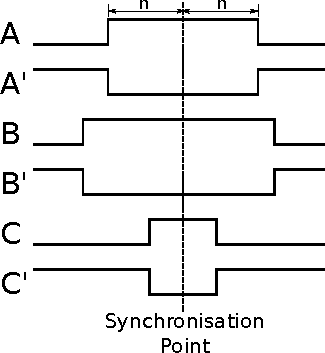
\includegraphics{images/pwmFig.pdf}
\caption{Centrally Synchronised PWM}
\label{fig_PwmOutputExample}
\end{center}
\end{figure}


\subsection{Configuration}
The PWM module has three modes of operation defined, plus a number of other options. The modes are defined in \verb=dsc_config.h= that is part of the application code. 

\subsubsection{PWM Modes}
The PWM operation mode can be one of three of the following options:

\begin{itemize}
\item \verb=PWM_INV_MODE= - This operates a three leg 180 degree inverter by ensuring that the HI and LO sides of the inverter are switched in a complementary manner
\item \verb=PWM_NOINV_MODE= - Simple three channel PWM that operates three channels as above without the inversion
\item \verb=PWM_BLDC_MODE= - Basic BLDC commutation mode operates a three leg inverter by switching the HI side and then applying PWM to the low side of the inverter to achieve simple commutation
\end{itemize}

\subsubsection{Dead Time}
The dead time for \verb=PWM_INV_MODE= is defined using the \verb=PWM_DEAD_TIME= configuration. This is in units of 10ns when using the default reference clock of 100MHz.

\subsubsection{PWM Resolution}
PWM resolution is defined using \verb=PWM_MAX_VALUE=. The value defined here sets the frequency of the PWM. The relationship between \verb=PWM_MAX_VALUE=, \verb=XS1_TIMER_HZ= and PWM frequency ($PWM\_FREQ$) is defined in equation \ref{eqn_PwmFreq}. \verb=XS1_TIMER_HZ= is defined at compile time by the \verb=ReferenceFrequency= identifier in the project XN file. By default this reference frequency is 100MHz so \verb=XS1_TIMER_HZ= would have a value of 100,000,000.

\begin{equation}\label{eqn_PwmFreq}
PWM\_FREQ = \frac{XS1\_TIMER\_HZ}{PWM\_MAX\_VAL} 
\end{equation}

So with an example value of \verb=PWM_MAX_VALUE= being 4096 (12 bit resolution), the \verb=PWM_FREQ= will be 24,414Hz.

\subsubsection{Locking the ADC trigger to PWM}
In some implementations it is desirable to lock the ADC conversion trigger to the PWM. This allows the system to sample the ADC at a specific point in the PWM period (such as when the lower leg is guaranteed to be on). This is enabled using the \verb=LOCK_ADC_TO_PWM= definition.

\subsubsection{Default PWM Configuration}
The default configuration for the demonstration application is as follows. 

\begin{lstlisting}
#define PWM_INV_MODE 1
#define PWM_DEAD_TIME 10
#define PWM_MAX_VALUE 4096
#define LOCK_ADC_TO_PWM 1
\end{lstlisting}

\subsection{PWM Server Usage}
The usage for each mode is described below. The PWM server needs to be instantiated on the same core as the PWM client. The following is required to be included.

\begin{lstlisting}
#include "pwm_service.h"
\end{lstlisting}

\subsubsection{Inverter Mode}
To instantiate the PWM service the function described in the listing below needs to be called for the \verb=PWM_INV_MODE= and \verb=LOCK_ADC_TO_PWM= combination.

\begin{lstlisting}
void do_pwm( chanend c_pwm, chanend c_adc_trig, 
	in port dummy_port, 
	buffered out port:32 p_pwm[],  
	buffered out port:32 p_pwm_inv[], 
	clock clk);
\end{lstlisting}

\verb=chanend c_pwm= is the channel used to communication with the client side.

\verb=chanend c_adc_trig= is the channel used to communicate the triggering of the ADC conversion to the ADC thread

\verb=in port dummy_port= is an unused port that is used to consistently trigger the ADC conversion. This port can overlap other used ports at it is never written to and the input value is never used.

\verb=buffered out port:32 p_pwm[]= and \verb=buffered out port:32 p_pwm_inv[]= are arrays of 1 bit ports with an array length of 3 that are used for the HI and LO sides of inverter respectively.

\verb=clock clk= is the clock block that the PWM thread uses for timing output.

If \verb=LOCK_ADC_TO_PWM= is not defined then the following call is used.

\begin{lstlisting}
void do_pwm( chanend c_pwm,
	buffered out port:32 p_pwm[],  
	buffered out port:32 p_pwm_inv[], 
	clock clk);
\end{lstlisting}

The argument definitions are as above.

\subsubsection{Simple three channel PWM mode}

This mode is currently only used for testing. It is similar in operation to the inverter mode, but does not have ADC locking functionality and operates only half of the inverter. 

\subsubsection{Basic BLDC commutation mode}
This mode of operation is slightly different to the others as it is designed for simple commutation of a brushless DC motor. An example of the output of this mode is shown in figure \ref{fig_PwmBldcMode}

\begin{figure}[h]
\begin{center}
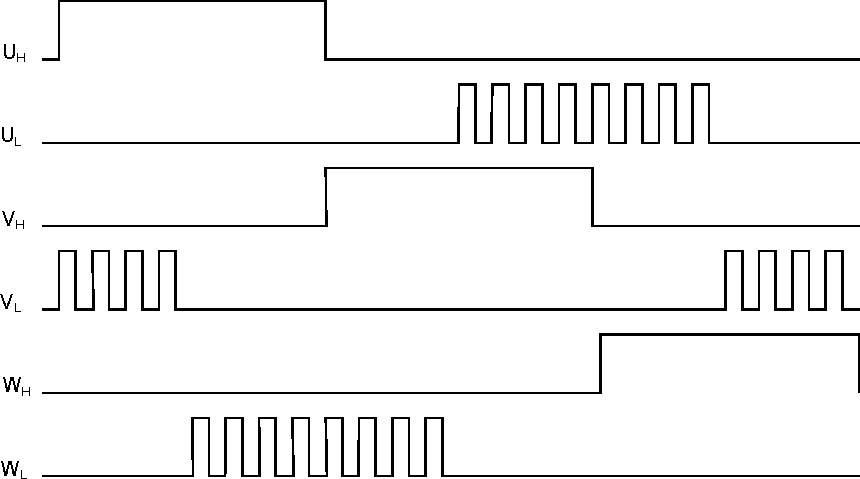
\includegraphics[width=0.9\textwidth]{images/bldcpwm.pdf}
\caption{BLDC Mode PWM Output}
\label{fig_PwmBldcMode}
\end{center}
\end{figure}

To instantiate the PWM service in this mode the following function needs to be called.

\begin{lstlisting}
void do_pwm( chanend c_pwm, 
	buffered out port:32 p_pwm[], 
	clock clk);
\end{lstlisting}

\verb=chanend c_pwm= is the channel used to communication with the client side.

\verb=buffered out port:32 p_pwm[]= is an array of 1 bit ports with an array length of 3 that are used for the HI or LO sides of the inverter respectively.

\verb=clock clk= is the clock block that the PWM thread uses for timing output.

\subsection{PWM Client Usage}
The PWM client functions must be operated on the same core as the server. The usage of the client functions in the various operational modes are described below. The following must be included to call the client functions.

\begin{lstlisting}
#include "pwm_cli.h"
\end{lstlisting}

\subsubsection{Inverter Mode}
The only call required to update the PWM values that are currently being output is listed below. It takes only two arguments, the channel to the PWM server and an array of size three containing unsigned integers that must be between 0 and \verb=PWM_MAX_VALUE=.

\begin{lstlisting}
void update_pwm( chanend c, unsigned value[]);
\end{lstlisting}

This function will process the values and pass them to the PWM service thread.

\subsubsection{Simple three channel PWM mode}

See details above for the Inverter Mode.

\subsubsection{Basic BLDC commutation mode}
The basic BLDC commutation mode client operates slightly differently to achieve the waveform shown in figure \ref{fig_PwmBldcMode}. The function call listed below must be utilised. 

Only a single output is active at any one time and this channel must be identified using the \verb=pwm_chan= argument, this is a value between 0 and 2. The corresponding leg of the inverter needs to be switched manually in the control thread. Please refer to the \verb=app_basic_bldc= application and associated documentation. 

\begin{lstlisting}
void update_pwm( chanend c, 
	unsigned value, 
	unsigned pwm_chan );
\end{lstlisting}

\subsection{PWM Service Implementation}
The PWM service is designed as a continuously running loop that cannot be blocked. This is important to ensure continuous output as stalling an output on an inverter in any application could result in serious failure of the appliance that is being driven.

To achieve the behaviour needed the PWM services are all written in assembly language. This is done to achieve a fine grained control over the instruction sequences required to load up the buffers in the ports and also the port timers.

The PWM service pulls the required data for outputting to the ports from a shared memory location. This is a `double buffered' scheme where the client will update the memory area that is not currently in use and then inform the service via a channel which memory location it should look at for the output data. The update sequence is looked at in more detail in the discussion of the client implementation.

Operation of the full inverter mode is the most complex, so this will be the case that is dealt with here. The other modes (simple three channel and BLDC commutation) are derived from this inverter implementation and thus do not need separate explanation.

We will therefore be covering the operation that is found in \newline \verb=module_dsc_pwm/src/dsc/pwm_svr/inv_svr/=. 

\subsubsection{PWM service port initialisation (pwm\_service\_inv.xc)}
This file achieves a number of functions. The primary function is a wrapper that is called to start the PWM service running. This configures the port and then enters the main loop for the PWM service.

\begin{lstlisting}
#if LOCK_ADC_TO_PWM
void do_pwm_inv( chanend c_pwm, 
    chanend c_adc_trig, 
    in port dummy_port, 
    buffered out port:32 p_pwm[], 
    buffered out port:32 p_pwm_inv[], 
    clock clk)
#else
void do_pwm_inv( chanend c_pwm, 
    buffered out port:32 p_pwm[],  
    buffered out port:32 p_pwm_inv[], 
    clock clk)
#endif
{

  t_out_data pwm_out_data0, pwm_out_data1, pwm_out_data2;
  unsigned buf;

  /* configure the ports */
#if LOCK_ADC_TO_PWM
  // has a dummy port for ADC config
  do_pwm_port_config_inv_adc_trig( dummy_port, 
                                   p_pwm, p_pwm_inv, clk );
#else
  do_pwm_port_config_inv( p_pwm, p_pwm_inv, clk);
#endif

  /* wait for initial update */
  c_pwm :> buf;

  while (1)
  {
  #if LOCK_ADC_TO_PWM
    buf = pwm_op_inv( buf, p_pwm, p_pwm_inv, c_pwm, 
                      c_adc_trig, dummy_port );
  #else
    buf = pwm_op_inv( buf, p_pwm, p_pwm_inv, c_pwm );
  #endif
  }

}
#endif
\end{lstlisting}

The first function calls are the initial configuration of the ports. This is done in \verb=do_pwm_port_config_inv( ... )= or \verb=do_pwm_port_config_inv_adc_trig( ... )= depending on whether the option of ADC triggering has been selected. The function used to configure the ports with the ADC triggering is merely a simple extension of the operation of the mode without ADC triggering and so will be explained here.

\begin{lstlisting}
static void do_pwm_port_config_inv_adc_trig( in port dummy, 
  buffered out port:32 p_pwm[], 
  buffered out port:32 p_pwm_inv[], 
  clock clk )
{
  unsigned i;

  for (i = 0; i < PWM_CHAN_COUNT; i++)
  {
    configure_out_port(p_pwm[i], clk, 0);
    configure_out_port(p_pwm_inv[i], clk, 0);
    set_port_inv(p_pwm_inv[i]);
  }

  /* dummy port used to send ADC trigger */
  configure_in_port(dummy,clk);

  start_clock(clk);
}
\end{lstlisting}

Firstly three legs of the inverter drive are configured to be attached to the clock block and have an initial output of 0. This is deemed to be a safe start-up configuration as all drives are switched off.

Then, in the loop, the `inverted' ports are configured to output the inverse or complementary of the data that is put into the buffers. This means that only a single data set need be maintained and removes the need for inverting the data using the instruction set as this is done by the port logic.

Following the loop that sets up the individual PWM channels is the configuration for the ADC triggering port. This is an input port that is attached to the same clock block as the PWM output ports. An input port that overlaps other in use ports (as described in the usage section above) will not affect their operation. The dummy port is just used for timing synchronisation when signalling the ADC.

Finally the clock block is started.

Once the ports have been configured the output will remain in the initialised state until the thread receives notification from the client thread that data is available in the shared memory for output. It is important to wait for the first client update otherwise there is a risk of output uninitialised data which may damage the drive circuitry.

Once this information is received the main loop is entered.

\subsubsection{PWM service main loop (pwm\_op\_inv.S)}
The operation of the main loop is best described visually as in the flow chart shown in figure \ref{fig_PwmMainLoopFlow}. The entries in the flow chart relate directly to the labels within the main loop. 

A brief overview of each part of the main loop are given below. These should be consulted alongside the comments that reside in the code itself.

\begin{figure}[p]
\begin{center}
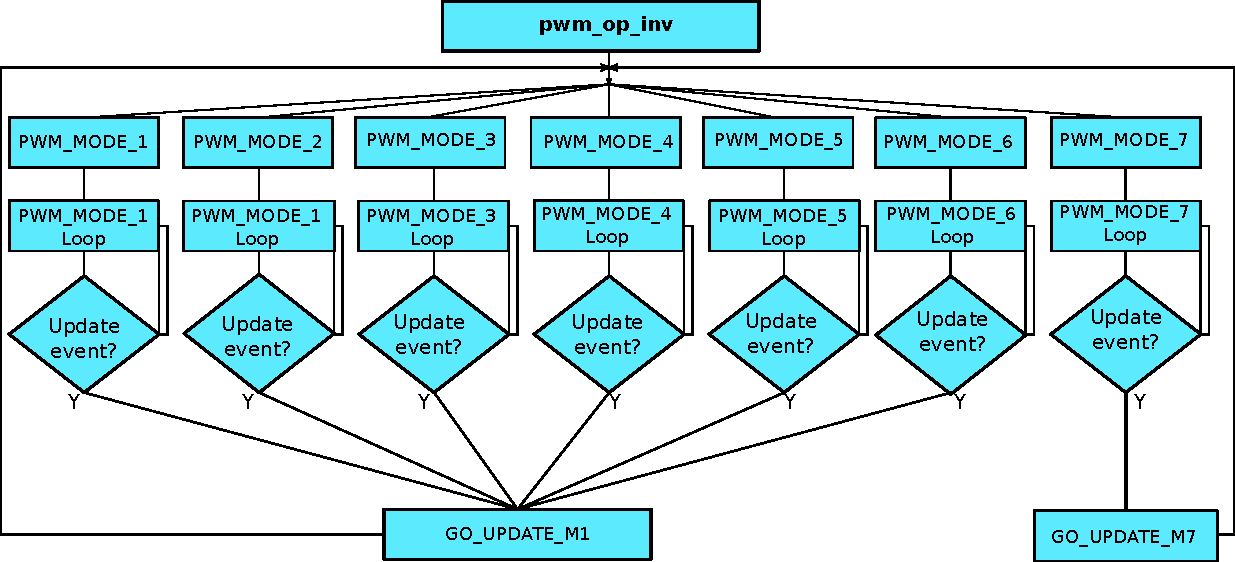
\includegraphics[width=0.9\textheight, angle=90]{images/pwm_loop.pdf}
\caption{PWM Main loop flow chart}
\label{fig_PwmMainLoopFlow}
\end{center}
\end{figure}

The code begins at the \verb=pwm_op_inv= entry point. This begins by running a standard callee save. This preserves any registers that we will clobber as part of the operation of this function. The arguments to the function are then stored on the stack itself in \verb=sp[8:11]=. This ensures we have access to them later.

Following this the registers are moved around into the configuration we require and data is read from the \verb=t_data_out= structure after calculating the appropriate pointers. The port resource IDs are then loaded into registers and the `mode' of operation is read and the port timer read to initialise the synchronisation point.

The code then branches to the appropriate mode according to the mode value that has been read from the data structure provided to it by the client.

\paragraph{Why all these loop modes?} It is worth discussing at this point why there are different loop modes and what they achieve. The nature of the central synchronisation point means that there are very rare times when the edges of the PWM coincide - from an electrical noise standpoint this is beneficial, but from and implementation standpoint it complicates things slightly.

To achieve the required output efficiently using the ports the buffers are used to create the extremely short or long pulses as shown in figure \ref{fig_PwmPortBuffering}. The green boxes indicate a buffer of data that is output from the port.

\begin{figure}[h]
\begin{center}
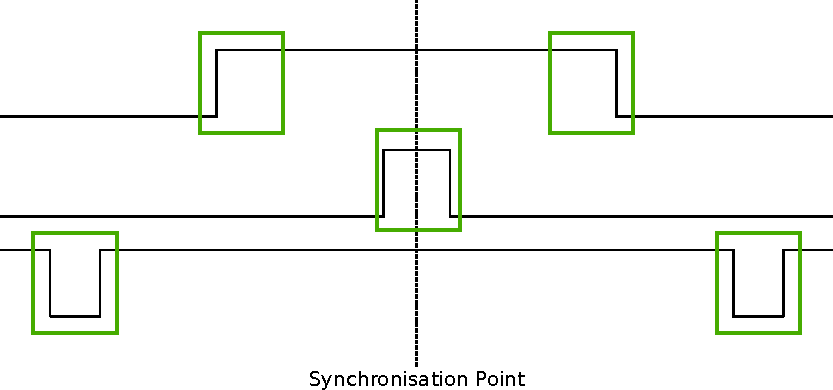
\includegraphics[width=0.9\textwidth]{images/bufferedPWM.pdf}
\caption{PWM Buffered Port Output}
\label{fig_PwmPortBuffering}
\end{center}
\end{figure}

This method of output requires a combination of one or two buffer outputs depending on the length of these pulses. Rather than calculate these during runtime the client will ascertain the particular combination of outputs required and then will define the mode. The different buffering output modes are individually implemented to reduce branching overhead within the loop.

At the entrance to the loop mode (taking \verb=PWM_MODE_4= as the working example) the mode value is replaced with the channel end resource ID. We then enter the core of the PWM service loop. The loop will setup each of the ports in sequence, calculating the appropriate port timer value from the data set that is provided by the client.

When the option to lock the ADC to PWM is required then the system will block on the \verb=in= instruction while it waits for the timer on the dummy port. Once the port timer reaches the required value the thread will output the token to the ADC thread.

If the ADC to PWM lock is not utilised then the thread will pause on the next \verb=setpt= instruction until that particular port timer value is met and the data is output. The ports are loaded in reverse order to turn them off at the correct time. Once all of the channels are reloaded the thread will check for data on the update channel. If data is found then it will immediately enter \verb=GO_UPDATE_M1= otherwise it will continue through the loop calculating the next synchronisation point and looping back to the top of the output sequence.

If the system branches to update then it will execute a sequence very similar to the entry of the function, reading the data out of the data structure and setting up the relevant memory pointers. The update for \verb=PWM_MODE_[1:6]= loops are all the same. In the case of \verb=PWM_MODE_7= the update sequence is slightly different due to the fact that the even is likely to occur when one of the channels is high. This means that a further output is required before receiving the update from the client.

\subsection{PWM Client Implementation}
The PWM client is required to do a number of functions to provide the correct data to the PWM service that outputs the correct values and timings to the ports. The PWM client must:

\begin{itemize}
\item Calculate the output values
\item Calculate the timing values (taking into account dead time)
\item Sort the ports into time order
\item Ascertain the loop mode required
\item Maintain the shared data set, including which buffer is in use and which one can be updated
\end{itemize}

Taking the inverter mode as our working example (located in \newline \verb=module_dsc_pwm/src/dsc_pwm_cli/pwm_cli_inv=) the function \verb=update_pwm(...)= first saves the PWM values for later use and then initialises the channel ordering array to assume a sequential order of output. 

Following this the calculation of the timings and output values are done for each of the channel. This is done by passing the relevant PWM value and data set references to the \verb=calculate_data_out_ref(...)=. This function also ascertains the type of output which can be one of three values \verb=SINGLE=, \verb=DOUBLE= and \verb=LONG_SINGLE=.

Once the calculations for each of the PWM channels is completed they can be ordered. This is done using the \verb=order_pwm(...)= function. This orders the values in the channel ID buffer and also works out the loop mode that is required.

When the values have been ordered and the loop mode calculated the buffer number is passed to the PWM service to indicate an update.

